%============================
%User Management
%============================
\subsection{User Management}
This module is responsible for reading data from the client user database. It will do this by making use of ldap.js. This module will also retrieve the privileges a user has from the system's internal database.

\subsubsection{Scope}
The scope of the Project module is shown in the figure below:
	\begin{figure}[H]
	    	\centering
	    	\fbox{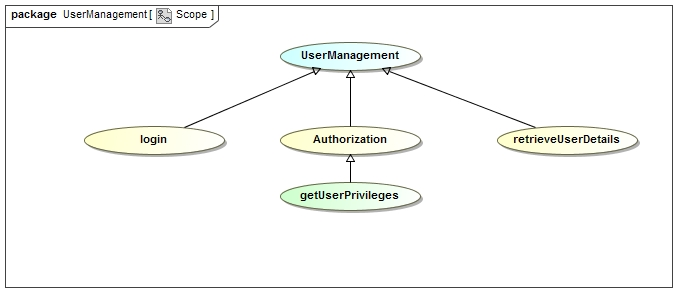
\includegraphics[width=1.0\textwidth]{UserManagementScope}}
	    	\caption{User Management Scope}
	    	\label{fig:UserManagementScope}
   	\end{figure}
\paragraph{Test}
\subsubsection{Use cases}

\paragraph{Login - priority: critical}
Takes user's credentials to log him into the system.

\paragraph{Authorize - priority: critical}
Authorizes users with the right privileges to do what is requested.

\paragraph{retrieveUserDetails - priority: important}
This will get the details from the both the external and internal databases, to supply details to other modules in system as they need it.

\subsubsection{Domain model}

%============================
%Project
%============================
\subsection{Project}
The project module is responsible for the representation and persistence of all projects that the system will use to do the estimations on. This module will allow for complex projects to be created, as well as to be updated. A project is represented as a tree, consisting of a top-level project node and lower-level task nodes.

\subsubsection{Scope}
The scope of the Project module is shown in the figure below
	\begin{figure}[H]
	    	\centering
	    	\fbox{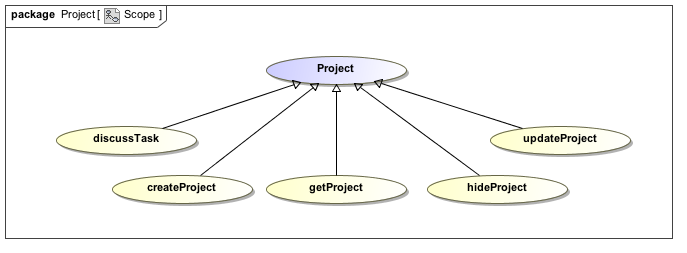
\includegraphics[width=1.0\textwidth]{projectScope}}
	    	\caption{Project Scope}
	    	\label{fig:Project_Scope}
   	\end{figure}
\subsubsection{Use cases}

\paragraph{Create a project - priority: critical}
Users with sufficient privileges can create projects. This will persist the project to the database.

\begin{itemize}
	\item Services contract:\\ \\
	The createProjectRequest contains the name of the project as well as the user who is creating the project. The function will allow the user to expand on the project in order to build a comprehensive project tree.
	\begin{figure}[H]
    	\centering
    	\fbox{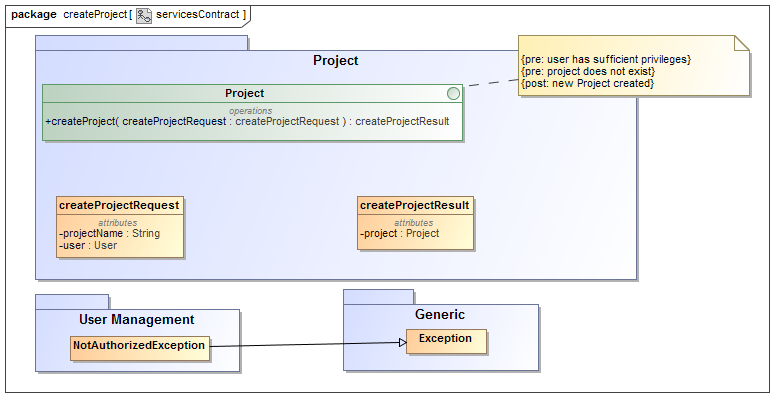
\includegraphics[width=1.0\textwidth]{servicesContractcreateProject}}
    	\caption{createProject services contract}
    	\label{fig:createProject_services_contract}
   	\end{figure}
\end{itemize}

\paragraph{Get project - priority: critical}
Users with sufficient privileges can retrieve projects to view them, or to be used for other purposes. This use case must thus return a representation of the project-tree, and not produce the output of the project tree.

\begin{itemize}
	\item Services contract:\\ \\
	The getProjectRequest contains the name of the Project that must be retrieved. The getProjectResult contains the Project that has been identified by the projectName.
	\begin{figure}[H]
    	\centering
    	\fbox{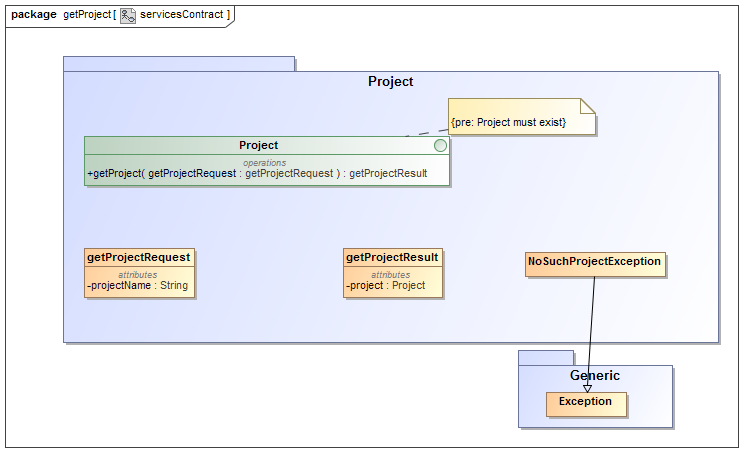
\includegraphics[width=1.0\textwidth]{servicesContractgetProject}}
    	\caption{getProject services contract}
    	\label{fig:getProject_services_contract}
   	\end{figure}
\end{itemize}

\paragraph{Hide project}
Projects can be effectively deleted by hiding them, seeing as projects are not physically removed from the database. This action can only be done by authorised user.

\begin{itemize}
	\item Services contract:\\ \\
	The hideProjectRequest contains a reference to the Project that must be hidden, which can be obtained by calling the getProject function.
	\begin{figure}[H]
    	\centering
    	\fbox{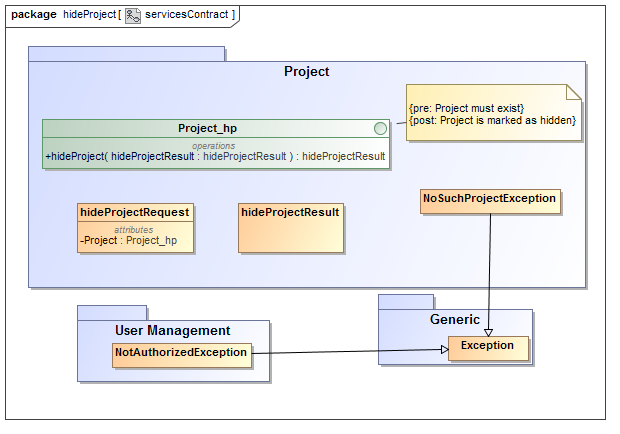
\includegraphics[width=1.0\textwidth]{servicesContracthideProject}}
    	\caption{hideProject services contract}
    	\label{fig:hideProject_services_contract}
   	\end{figure}
\end{itemize}


\paragraph{Update project - priority: critical}
This enables users to update projects, if they have sufficient privileges, by adding or removing task nodes to and from the project tree.

\begin{itemize}
	\item Services contract:\\ \\
	The updateProjectRequest contains a reference to the project that needs to be update which can be obtained by making use of the getProject functionality. The updateProjectRequest also contains a reference to the updated project, which can either be an entirely different project, or the same project as represented by oldProject, but with some changes applied to it.
	\begin{figure}[H]
    	\centering
    	\fbox{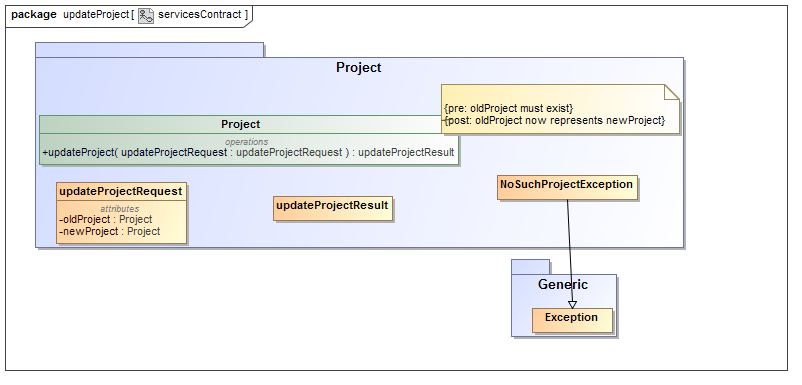
\includegraphics[width=1.0\textwidth]{servicesContractupdateProject}}
    	\caption{updateProject services contract}
    	\label{fig:updateProject_services_contract}
   	\end{figure}
\end{itemize}

\subsubsection{Domain model}
The domain model for the Project module requires that tasks being created and added to the tree, be persisted. Each project holds a reference to its parent, which is also of type Project. Furthermore, each Project holds a list of all its children, which once again, are also of type Project. Each instance of Project is represented as a Task object, which contains references to estimations made on that specific task.
\begin{figure}[H]
	\centering
	\fbox{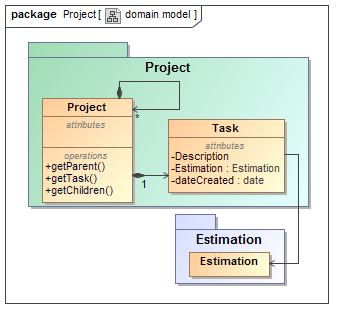
\includegraphics[width=0.5\textwidth]{projectdomainmodel}}
	\caption{Project domain model}
	\label{fig:Project_domain_model}
\end{figure}
%============================
%Estimation
%============================
\subsection{Estimation}
	The Estimation module will be responsible for handling all of the actions related to the estimation of a project. This involves allowing a user to place an estimate on a specific task as well as calculating the total estimation of a project.
\subsubsection{Scope}
	This is the estimation scope
	\begin{figure}[H]
	    	\centering
	    	\fbox{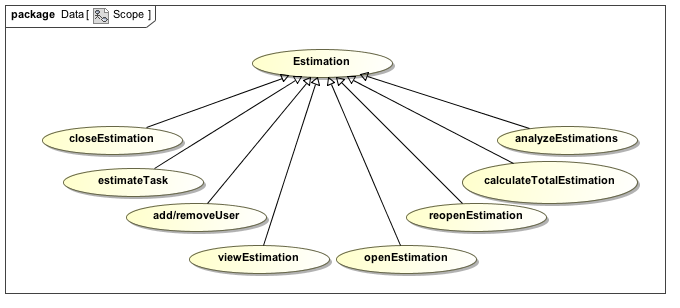
\includegraphics[width=0.5\textwidth]{Estimation_Scope}}
	    	\caption{Estimation Scope}
	    	\label{fig:Estimation_Scope}
   	\end{figure}
\subsubsection{Use cases}
	\paragraph{estimateTask - priority:critical}This system will allow a user to place an estimation on a task.
	\paragraph{calculateTotalEstimation - priority:critical}This system will traverse the project tree and calculate the total estimation of a project.
\subsubsection{Domain model}
%============================
%Report
%============================
\subsection{Report}
The Report module will do statistical analysis on the data as well as draw graphs of the estimation data. This module will be responsible for any analysis of the data. It's functionality will be expanded as development continues. This module will retrieve all the data it requires from the database and then process that data to produce an appropriate result.
\subsubsection{Scope}
The scope of this module will be accessible to any user at this point in the development, the only authorization that will take place is the initial log in of the user.
	\begin{figure}[H]
	    	\centering
	    	\fbox{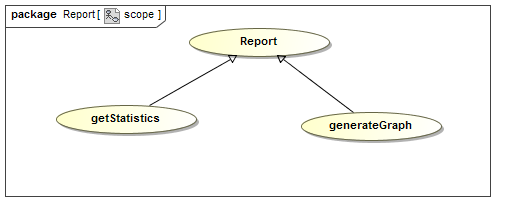
\includegraphics[width=0.8\textwidth]{Report_Scope}}
	    	\caption{Report Scope}
	    	\label{fig:Report_Scope.png}
   	\end{figure}
\subsubsection{Use cases}
	This section of the documentation will describe the use cases of the Report module.
	\paragraph{Statistical Analysis - priority:critical}
	User accessing this function will receive statistical analysis of the data for the chosen project.
	\paragraph{Generate Graphs - priority:critical}
	User accessing this function will receive a series of graphs of the data for the chosen project. 
\subsubsection{Domain model}

%============================
%Notification
%============================
\subsection{Notification}
This module will be responsible to notify all the users as required by the projects estimation. The estimation module will log a message request to the notification and add all the required users to notify.
\subsubsection{Scope}
This is the notification scope
	\begin{figure}[H]
	    	\centering
	    	\fbox{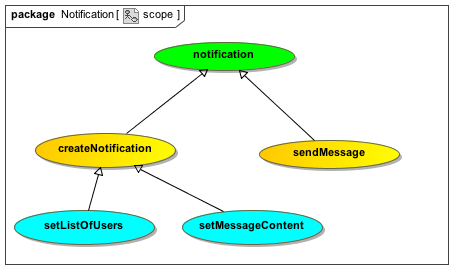
\includegraphics[width=0.8\textwidth]{Notification_Scope}}
	    	\caption{Notifications Scope}
	    	\label{fig:Notification_Scope}
   	\end{figure}
\subsubsection{Use cases}
The main purpose of notifications is to notify users with the required message. The estimation module will supply the list of users to notify and the contents of the message.
\paragraph{sendMesssage -- priority:niceToHave}
We will send the email to the destination address through the use of node mailer. 
\paragraph{createNotification -- priority:niceToHave}
The estimation module will create a notification request and send in to the notification module with the desired list of recipients.
	\begin{figure}[H]
	    	\centering
	    	\fbox{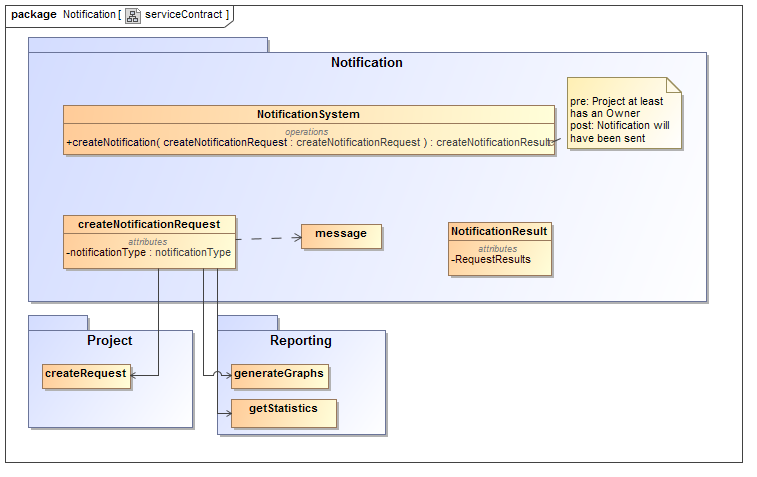
\includegraphics[width=0.8\textwidth]{NotificationServiceContract}}
	    	\caption{Notifications Service Contract}
	    	\label{fig:Notification_Service Contract}
   	\end{figure}
\subsubsection{Domain model}
	\begin{figure}[H]
	    	\centering
	    	\fbox{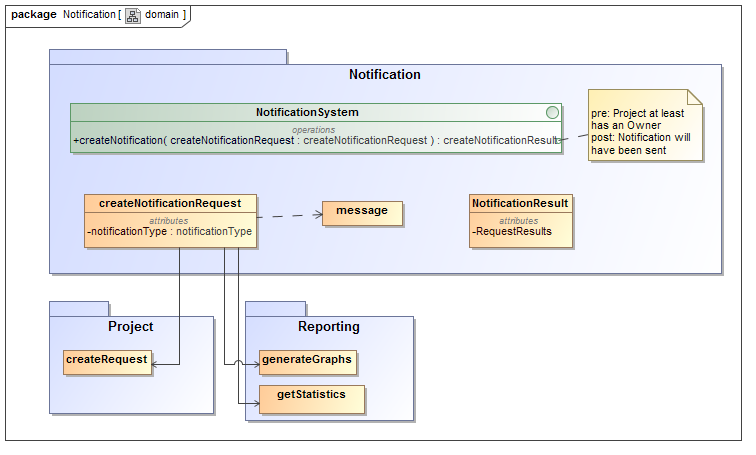
\includegraphics[width=0.8\textwidth]{NotificationDomain}}
	    	\caption{Domain Modelt}
	    	\label{fig:Domain Model}
   	\end{figure}
